\section{Basic Theory}
\subsection{The electric potential, Laplace's equation and the Uniqueness Theorem}
The usual task of electrostatics is to compute the electric field $\boldsymbol{E}$ given a 
stationary electric charge distribution $\rho_E{\boldsymbol{r'}}$
\begin{align}
   \label{electricField}
   \boldsymbol{E}(\boldsymbol{r}) 
   %&= \frac{1}{4 \pi \varepsilon_0} \int \frac{\boldsymbol{\hat{d}}(\boldsymbol{r'})}
                                              %{d(\boldsymbol{r'})^2} 
                                                            %\rho(\boldsymbol{r'}) d\!\boldsymbol{r'} 
                                                            %\\
   &= \frac{1}{4 \pi \varepsilon_0} \int \frac{\boldsymbol{r} - \boldsymbol{r'}}
                                              {\big|\boldsymbol{r} - \boldsymbol{r'}\big|^3} 
                                                           \rho(\boldsymbol{r'}) d\!\boldsymbol{r'}.
\end{align}
The notation for Eq.\eqref{electricField} can be shown in Figure \ref{fig:electricField}
and $\varepsilon_0 = 8.85 \cdot 10 ^{-12} \text{C}^2/\text{Nm}^2$ is the permittivity of free space
\cite[.~58-62]{Griffiths}.
%
\begin{figure}[h!]
  \centering
   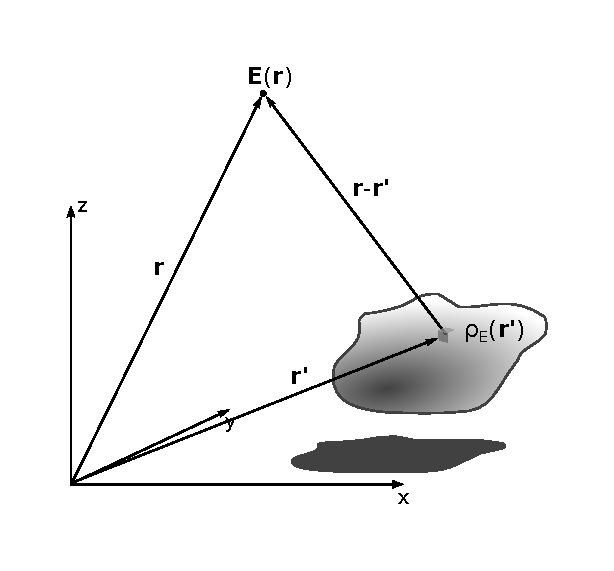
\includegraphics[width=0.5\textwidth]{../Figures/electricFieldcoord.pdf}
   \caption{
      The electric field $\boldsymbol E (\boldsymbol r)$ (at position $\boldsymbol r$)
      due to the charge distribution $\rho_E$ located at $\boldsymbol{r'}$.
   }
   \label{fig:electricField}
\end{figure}
%
However, it is usually simpler to calculate the electric potential $\Psi$
\begin{align}
   \label{electricPotential}
   \Psi(\boldsymbol{r}) 
   &= \frac{1}{4 \pi \varepsilon_0} \int \frac{1}{\big|\boldsymbol{r} - \boldsymbol{r'}\big|} 
                                                           \rho(\boldsymbol{r'}) d\!\boldsymbol{r'}
\end{align}
first and then calculate the electric field from
\begin{align}
   \boldsymbol{E} = - \nabla \Psi.
\end{align}
This might in some situations, where do do not necessarily know $\rho$ but only the total amount of 
charge, also be to tough to handle analytically. In situations like these it is better to use
Poisson's equation
\begin{align}
   \label{poisson}
   \nabla^2 \Psi= - \frac{1}{\varepsilon_o} \rho,
\end{align}
which together with appropriate boundary conditions, is equivalent to Eq.\eqref{electricPotential}.
Very often, we are interested in finding the potential containing no charge (because the charge is 
located on the outside of our region of interest. In such cases Eq. \eqref{poisson} reduces to
Laplace's equation (\cite{Griffiths}, p.110-111)
\begin{align}
   \label{laplace}
   \nabla^2 \Psi = 0.
\end{align}
According to the \textit{Uniqueness Theorems}, the solution to Laplace's equation is uniquely 
determined in some volume if the potential is specified on the boundary of the volume. This
easily extends to Poisson's equation by further requiring, in addition to the 
potential on the boundary, that the charge distribution throughout the region is known.
\\
\\
When considering conductors, charge are allowed to move freely and  might start to rearrange themselves,
leading to the \textit{Second uniqueness theorem}, which states that the potential in a given volume,
surrounded by conductors is uniquely determined if the total charge on each conductor is given.
\\
\\
The uniqueness theorem grants an enlarged mathematical freedom in the approach of finding the potential
of a region of space. This is because the boundary uniquely determines the potential in the region enclosed
region and any approach giving the correct boundary conditions would give you the correct potential 
function through Laplace's equation Eq. \eqref{laplace}. This allows the use of tricks, like for example
the classical \textit{method of images} (\cite{Griffiths}, p.116-121).





\subsection{Polarizability}
When a neutral atom is placed in an electric field $\boldsymbol{E}$, the field tries to rip the
atom apart by pushing the nucleus in the direction of the field and the electrons in the opposite direction.
Because of the attraction between the positive and negative charge within the atom, an equilibrium displacement
of the electrons compared to the nucleus is achieved, leaving the atom polarized and giving it a
dipole moment. The dipole moment can be approximated by
\begin{align}
   \boldsymbol{p} = \alpha \boldsymbol{E},
\end{align}
where $\alpha$ is the atomic polarizability and may depend on the detailed structure of the atom.
For more complicated situations, like an asymmetrical molecule, the gained dipole moment of the 
molecule does not necessarily have to be in the same direction as the applied electric field.
In such a case, the scalar polarizability in the expression above is replaced by a polarizability tensor
\begin{align}
   \boldsymbol{\alpha} = 
\begin{bmatrix}
   \alpha_{xx}   &   \alpha_{xy}  &  \alpha_{xz}  \\
   \alpha_{yx}   &   \alpha_{yy}  &  \alpha_{yz}  \\
   \alpha_{zx}   &   \alpha_{zy}  &  \alpha_{zz} 
\end{bmatrix}
.
\end{align}
In this way, an applied eletric field induces many dipole moments in a material. In addition,
any polar molecules will be subject to a torque, aligning it to the direction of the field.
These two mechanisms leads to the polarization $\boldsymbol{P}$ of the material
\begin{align}
   \boldsymbol{P} = \text{dipole moment per unit volume} = \varepsilon_0 \chi_e \boldsymbol{E}.
\end{align}
In the above expression, there has been assumed a linear dielectric media, where $\chi_e$ is the electric 
susceptibility and depends on the microscopic structure of the material, in addition to the external 
temperature (\cite{Griffiths},p.160-166, 179)



\subsection{Plasmons}

\subsection{\textbf{The Drude model} \cite{Hofmann} }
Defining the differences between the electrical properties of metals, semiconductors and insulators
is not a trivial matter. To put it simple, metals are good conductors, while semiconductors and 
insulators are not. However, semiconductors such as silicon conduct electrisity relatively well,
so the picture is not quite that simple.
\\
\\
A simple model, with fundamental importance regarding electrical conductivity, was suggested by
P. Drude in an attempt to explain the observed properties of metals. It is assumed that the 
electrons in a solid behave like a classical gas and do not interact with each other whatsoever.
Coloumb interaction is also neglected. This is known as the \textit{independent electron approximation}. 
The electron gas can be viewed as negatively charged particles bouncing about
immobile immobile positively charged ion cores. The only form of interaction in this model
are instantaneous collision between the electrons and ions; see Figure \ref{fig:DrudeModel}. 
The simplification of removing the Coloumb ion-electron interaction is called the 
\textit{free electron approximation}
%
\begin{figure}[h!]
  \centering
   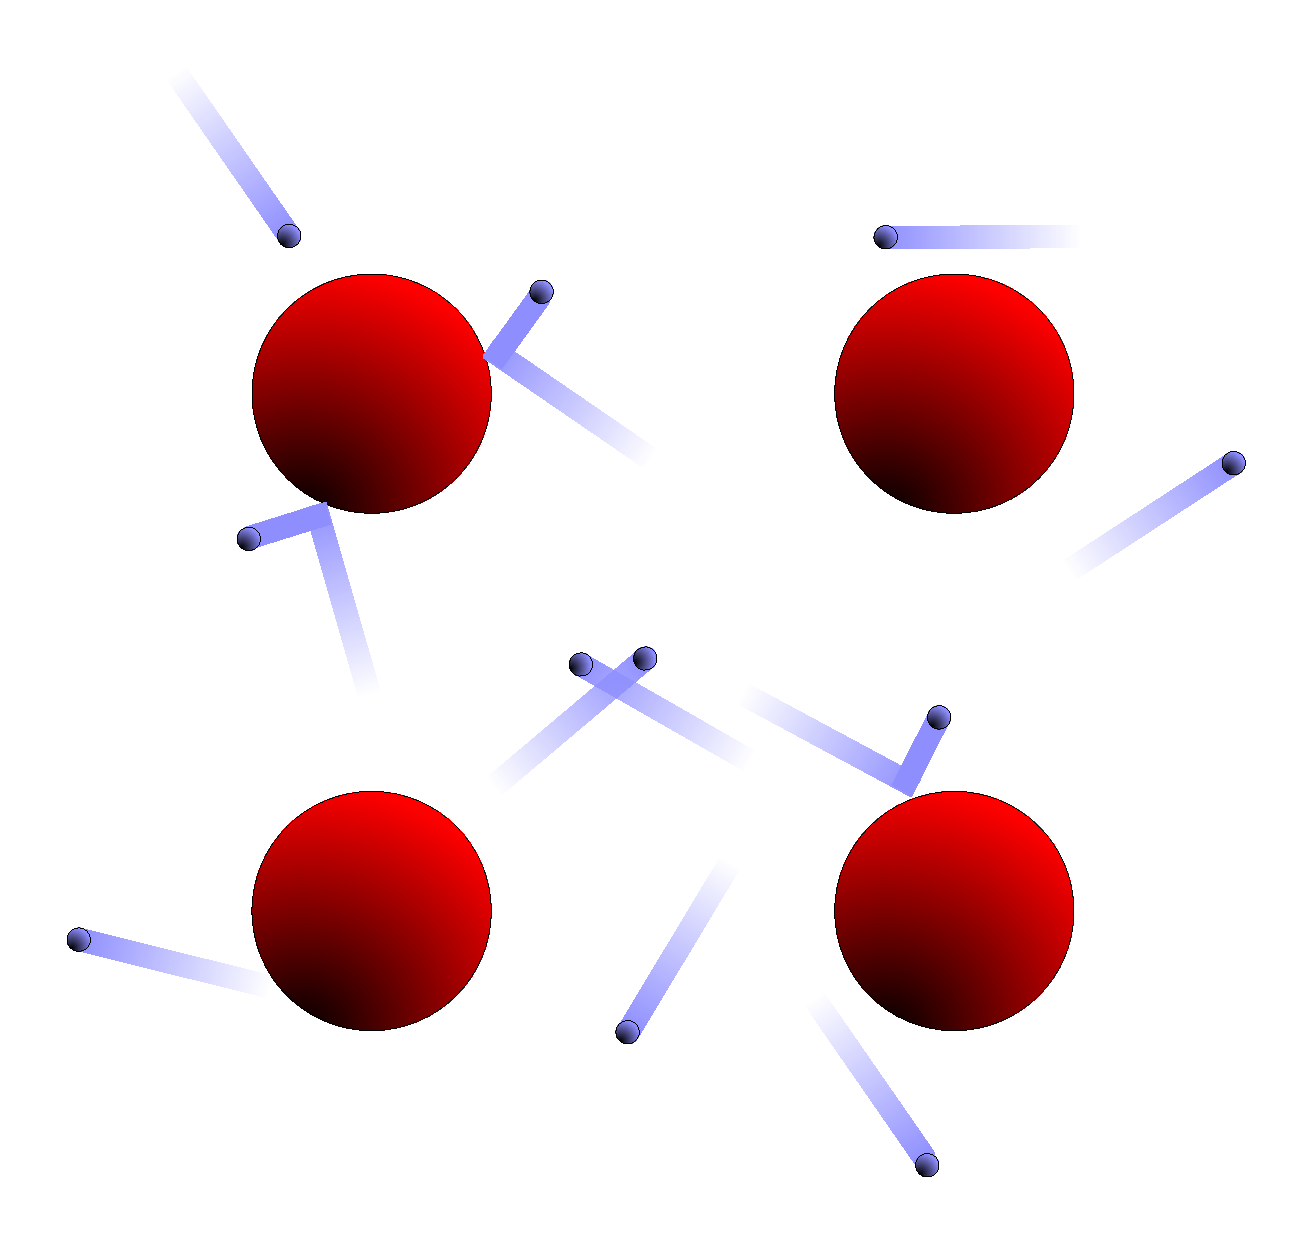
\includegraphics[width=0.5\textwidth]{../Figures/DrudeModel.pdf}
   \caption{ 
      The Drude model. A non-interacting electron gas (blue) is swirling around and colliding with 
      stationary positive ion cores (red). 
      Since all Coloumb forces are neglected together with electron-electron
      collsion, this ion-electron interaction is the only one being considered.
   }
   \label{fig:DrudeModel}
\end{figure}
%
The electrons reach thermal equilibrium with the lattice through the collisions, giving them
the kinetic energy:
\begin{align}
   \frac{1}{2}m_e v_t = \frac{3}{2}k_B T.
\end{align}
The average time between two collisions is called the relaxation time $\tau$, with the 
corresponding mean free path defined as $\lambda  = \tau v_t$. The probability for a 
electron to collide per unit time is assumed to be $1/\tau$. 
\\
\\
It is necessary to determine the conduction electron density $\rho_{c,e}$ in order to describe
properties such as electrical conductance. Assuming that every atom contributes 
every electron in its outermost shell $N_e$, e.g. that alkali metals contribute $N_e = 1$ and 
that earch alkaline earth metals contribute $N_e = 2$ etc. The number of atoms $N_a = \rho_m /m_a$, 
where $\rho_m$ is the density of the metal in [kg/m$^{-3}$] and $m_a$ is the atomic mass in [kg] 
(mass per atom).

\subsection{Conductivity; the Drude model}
Subjecting the drude metal of an electric field $\boldsymbol E$ will lead to a drift of the electrons
\begin{align}
   \frac{d \boldsymbol v}{dt} m_e = -e \boldsymbol E ,
\end{align}
where $e$ is the elementary charge. The solution is given by
\begin{align}
   \boldsymbol v (t) = \frac{-e \boldsymbol E t}{m_e}.
\end{align}
Assuming that the drift montion is destroyed in a collision, the average drift speed 
of the electrons become
\begin{align}
   \bar{\boldsymbol v }(t) = \frac{-e \boldsymbol E \tau}{m_e},
\end{align}
which is very slow compared to the thermal movement of the electrons $v_t$.
\\
\\
Considering an area $A$ perpendicular to the electric field, the amount of charge passing through 
the area is $-e n_e | \bar{\boldsymbol v} | A $ and the resulting current density would be
\begin{align}
   \boldsymbol j = n  \bar{\boldsymbol v} (-e) = \frac{n_e e^2 \tau}{m_e} \boldsymbol E \equiv \sigma \boldsymbol E = \boldsymbol E / \rho.
\end{align}
This is the familiar Ohm's law, with the conductivity 
\begin{align}
\sigma = \frac{n_e e^2 \tau}{m_e}
\end{align}
and the resistivity $\rho$. The $e^2$ dependence comes from the size of the pulling force
due to the electric field, i.e. how fast the particles move, and the other is how the same
charge, now moving, defines the current. This also means that we would get the same 
result for carriers with charge $e$ instead of $-e$, which would be the case for semiconductors
with positive holes.

\subsection{Optical reflectivity of drude metals}
The optical properties of materials are described by the complex refractive index $N(\omega)$ or 
the dielectric constant $\varepsilon(\omega)$. 
To explain the reflectivity of metals we can concider an electron in an electromagnetic 
field induced by an optical incident wave with wavenumber $q = 2\pi N/\lambda_0$, where 
$\lambda_0$ is the wavelength of the wave in free space.\\
If $\omega$ is low, we basically retain the DC behavior. However, if $\omega$ is so high that 
$1/\omega \ll \tau$, the electrons does not manage to react fast enough and the collisions with 
the ions altogether can be ignored (this is fulfilled for optical frequencies when $\tau=10^{-14}$s). 
The electrons can now be treated as completely free, and a single electron follows
\begin{align}
   m_e \frac{d^2x(t)}{dt^2} = -e E(t) = -e E e^{-i \omega t}.
   \label{freeElectronGas}
\end{align}
A good ansatz for the solution is setting $x(t) = xe^{-i \omega t}$, which mean that 
the electron is oscillating along with the electric field. This gives an amplitude of
\begin{align}
   x = \frac{eR}{m_e \omega^2}.
\end{align}
The corresponding polarization due to the dipole moment of $-ex$ for a solid with conduction electron
density $n_e$ is
\begin{align}
   P = -n_e ex = -\frac{n_e e^2E}{m_e \omega^2}.
\end{align}
From the constitutive relation
\begin{align}
   D = \varepsilon \varepsilon_0 E = \varepsilon_0 E + P,
\end{align}
we get that 
\begin{align}
   \varepsilon = 1 + \frac{P}{\varepsilon_0 E} = 1 - \frac{n_e e^2}{\varepsilon m_e \omega^2}
   \equiv 1 - frac{\omega_p^2}{\omega^2},
\end{align}
with the plasma frequency $\omega_p$ defined as
\begin{align}
   \omega_p = \frac{n_e e^2}{m_e\varepsilon_0}.
\end{align}
We can distinguish between two different cases and resulting outcome can
be seen from the the electromagnetic plane wave
\begin{align}
   \boldsymbol E (z,t) = \boldsymbol E_0 e^{i(2\pi N z/ \lambda_0 - \omega t)}.
\end{align}
In case 1) $\omega < \omega_p$ 
and $\varepsilon$ is a real and negative, $\varepsilon = \Re\{\varepsilon\} < 0$.
Therefore, $N = \sqrt{\varepsilon}$ is purely imaginary, and the wave penetrating the solid
is exponentially damped. Because Eq.\eqref{freeElectronGas} contain no inelastic properties, nothing
is absorbed. The light that is not transmitted into the medium must therefore, due to energy conservation, be
reflected back. 
For $\omega > \omega_p$, the dielectric constant is real and positive ,$\varepsilon = \Re\{\varepsilon\} > 0$,
and so is, followingly, the index of refraction. The result is a plane wave that propagates 
into the metal. This explains why metals are so reflective, or shiny. They are reflective for 
low-frequency light, but transparent for high-frequency light. The transition happens
at the plasma frequeny, which can be calculated solely from the conduction electron density of 
the metal. For most metals, the plasma frequency is in the far UV region, making them reflective 
in the visible range. Frequently, the plasma energy $\hbar \omega_p$ is used instead of the plasma frequency
$\omega_p$.

\subsection{Shortcomings of the Drude model}
The quenstionable assumptions of the Drude model is the removal of the electron-electron interaction
together with all the Coloumb forces. In addition, the assumption of treating the electrons as 
particles is not justified due to the fact that their de Broglie wavelength, in the case of thermal
electrons, is in the order of nanometers. The assumption would however only satisfy electrons moving
in structures much larger than the de Broglie wavelength.
\\
\\
The resulting conductivity of the model is not high enough at low temperatures, and is due to the
assumption of a fixed mean free path, given by the atomic spacing. Apparantly, at low temperature,
the electrons manage to sneak past the other electrons and ions. 
\\
\\
Also, the conductivity of alloys, in which impurities drastically reduce the conductivity, finds no
justification in the Drude model. 


\subsection{\textbf{Dielectrics}}
\subsection{Microscopic polarization}
There are several mechanismc causing microscopic electric dipole moments that lead to macroscopic 
polarization. E.g. displacement of electronic clouds and core, opposite displacement of the ions 
in a solid or
orientation of permanent dipoles such as water molecules, called orientational polarization.

\subsection{The local field}
To calculate the microscopic polarizability $\alpha$ of the atoms making up the solid, start with
the constitutive relation and assume that $\boldsymbol P$ can be written as the total dipole moment 
per unit volume
\begin{align}
   \boldsymbol P = (\varepsilon - 1 ) \varepsilon_0 \boldsymbol E = \frac{N}{V} \boldsymbol p = \frac{N}{V}\alpha \boldsymbol E.
   \label{nonLocalP}
\end{align}
Because a microscopic dipole within the solid does not simply feel the average electric field 
$\boldsymbol E$ but a microscopic local and stronger electric field $\boldsymbol E_{loc}$, the polarizability
can bot be correctly calculated from the above expression.
Without derivation, the approximate local field can be given by
\begin{align}
   \boldsymbol E_{loc} = \frac{1}{3}(\varepsilon + 2) \boldsymbol E.
\end{align}
So, with
\begin{align}
   \boldsymbol P = \frac{N}{V}\alpha \boldsymbol E_{loc}
\end{align}
and approximating the polarization $\boldsymbol P$ with Eq.\eqref{nonLocalP}, 
we get the so-called Clausius-Mossotti relation
\begin{align}
   \alpha = \frac{\varepsilon - 1}{\varepsilon + 2} \frac{3 \varepsilon_0 V}{N},
\end{align}
relating the atomic polarizabiliy to the dielectric constant.

\subsection{Frequency dependence of the dielectric constant}
The frequency dependent permittivity  $\varepsilon (\omega)$ is usually called the dielectric function.
For insulators, $\varepsilon(\omega)$ is complex and energy can be resonantly transferred to the solid
for certain frequencies. $\varepsilon(\omega)$ implies a frequency dependence of the refractive
index $N(\omega)$. Most of the frequency dependence can be explained by a simple idea 
combined with knowledge about the polarization mechanisms and how the different polarization mechanisms
manages to keep up with the oscillating electric field. E.g. orientation polarization and ionic polarization
does not manage to oscillate fast enough at higher frequencies, while the atomic polarization will, see
Figure \ref{fig:polarizationContribution}.
%
\begin{figure}[h!]
  \centering
   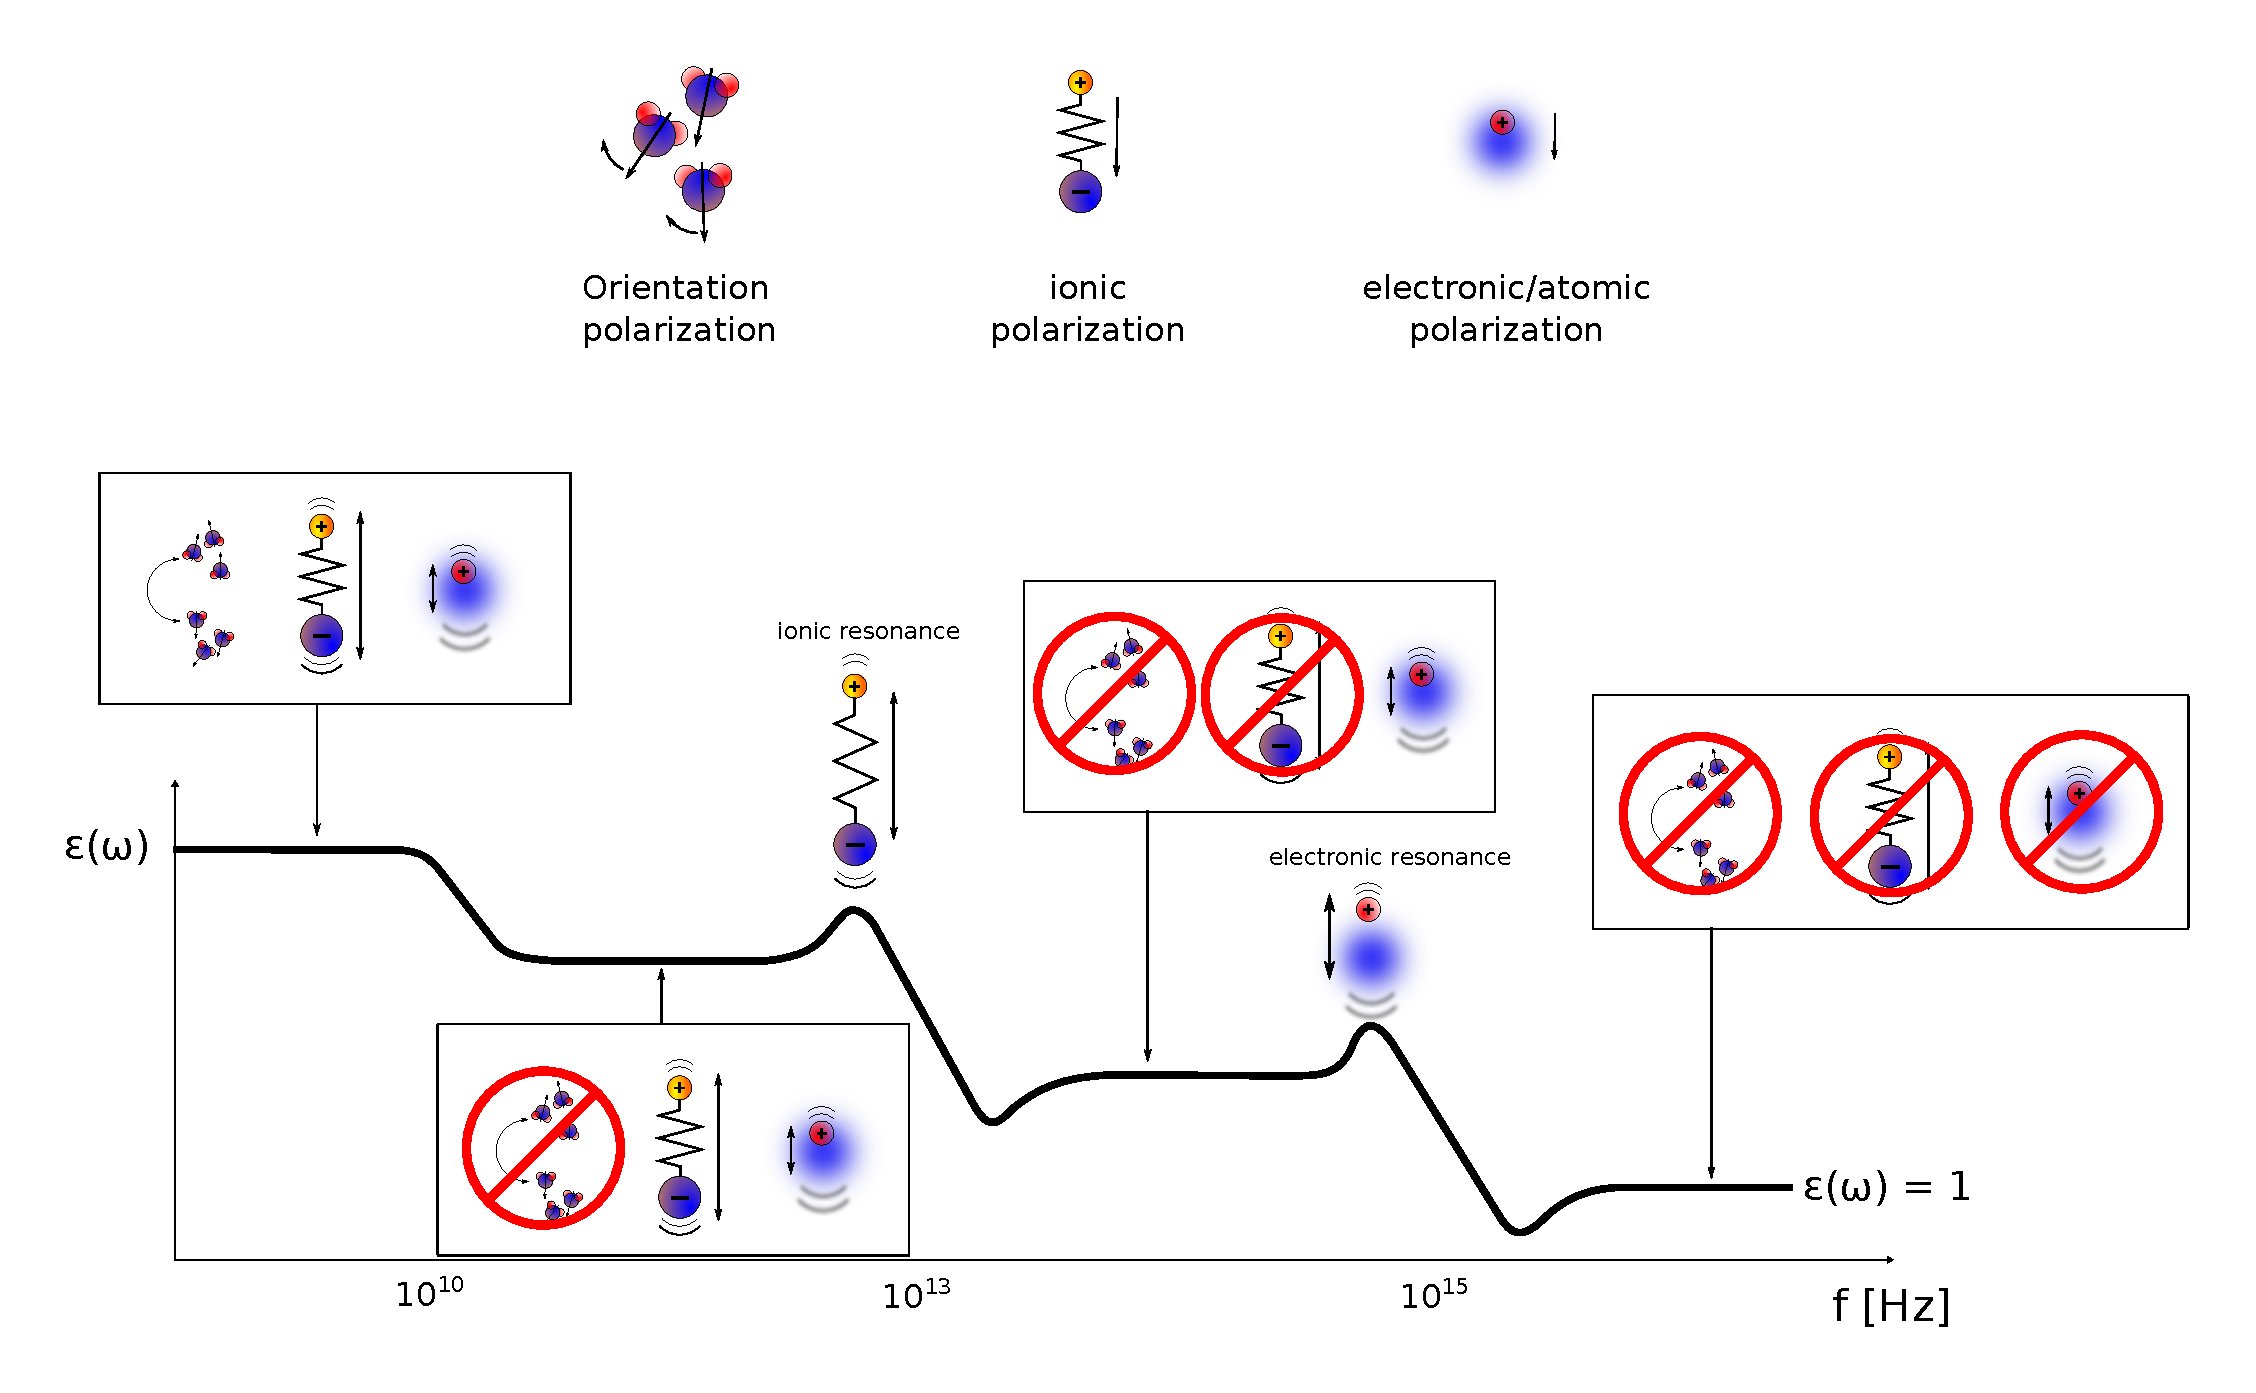
\includegraphics[width=1.0\textwidth]{../Figures/polarizationContributionToPermittivity.pdf}
   \caption{ 
      The contribution of orientation, ionic and electronic polarization. As the frequency
      of the applied electric field increases, the different polarization mechanisms fail to remain in 
      step with the field when above a characteristic frequency. At sufficiently high 
      frequencies the material no longer manages to polarize and the dielectric constant drops 
      to 1, corresponding to the permittivity of free space. Figure is adapted from 
      \cite{cambdridgePermittivityPage}.
   }
   \label{fig:polarizationContribution}
\end{figure}
%
\\
\\
For a quntitative description of the frequencydependence of $\varepsilon$ we can consider a simplified
version of ionic vibration.
Light can couple to optical phonons, e.g in ionic crystals where the phonons correspond to
an out-of-phase virbation of the positive and negative ions in the unit cell. 
These vibrations can be approximated by independent harmonic oscillators driven by an electric field
$E ^{-i\omega t}$, with one such oscillator per unit cell of the crystal. Each oscillator have a 
resonant frequency of $\omega_o = (2\gamma/M)^{1/2}$, where $\gamma$ is the force constant and
$M$ is the reduced mass of the two ions. The motion is damped by a term proportional to the velocity
$\eta d\!x\!/\!d\!t$ and represents the excitation of other vibrations in the material,
due to the large displacement. 
The resulting equation of motion is that of a driven harmonic oscillator with damping
\begin{align}
   \frac{d^2x}{dt^2} + \eta \frac{dx}{dt} + \omega_0^2 x = \frac{eE}{M}e^{-i\omega t}.
\end{align}
A good ansatz for the solution is 
\begin{align}
   x(t) = Ae^{-i \omega t},
\end{align}
resulting in the amplitude
\begin{align}
   A &= \frac{eE}{M} \frac{1}{\omega_0^2 - \omega^2 - i \eta \omega}  \\
     &=  \frac{eE}{M} \Bigg[ \frac{\omega_0^2 - \omega^2}{(\omega_0^2 - \omega^2)^2 +\eta^2 \omega^2} 
+ \frac{i\eta \omega}{(\omega_0^2 - \omega^2)^2 + \eta^2 \omega^2} \Bigg]
\end{align}
Using this as the ionic vibration, we can calculate the total polarization for a crystal with
$N$ unit cells and volume V. Considering only one type of ions with a density $N/V$ and effective
atomic polarizability $\alpha$, assuming both ionic and atomic polarization, $P_i(\omega)$, $P_a(\omega)$,
the result reads
\begin{align}
   P(\omega) = P_i(\omega) + P_a(\omega) = \frac{N}{V}eA(\omega)e^{-i \omega t} + \frac{N}{V}\alpha E e^{-i \omega t}.
\end{align}
When dealing with two types of ions like in a NaCl crystal, the different polarizabilities can be
taken care of by a suitable definition of $\alpha$. The resulting dielectric function can be calculated
from
\begin{align}
   \varepsilon_0 \varepsilon (\omega) E(\omega) = P(\omega) + \varepsilon_0 E(\omega),
\end{align}
giving
\begin{align}
   \varepsilon (\omega) &= \frac{P(\omega)}{\varepsilon_0 E e^{-i \omega t}} + 1  \\
                        &= \frac{NeA(\omega)}{V\varepsilon_0} + \frac{N \alpha}{V \varepsilon_0} + 1 \\
                        &= \frac{NeA(\omega)}{V\varepsilon_0} + \varepsilon\!_{_{opt}}.
\end{align}
Here, $\varepsilon_{opt}$ is the high frequency or optical limit, where the fields move to quickly for the 
ions to respond and $P_i(\omega) = 0$, i.e.
\begin{align}
   \varepsilon\!_{_{opt}} = \lim_{\omega\to\infty}\varepsilon (\omega)  
   = \frac{N \alpha}{V \varepsilon_0} + 1.
\end{align}
Plugging in the expression for $A(\omega)$ the real and complex values of the dielectric function 
$\varepsilon (\omega) = \varepsilon\!_{_{\Re\! e}} \!\! (\omega) + i \varepsilon\!_{_{\Im\! m}} \!\! (\omega)$ may be
written as
\begin{align}
   %\Re\! e [ \varepsilon (\omega) ]  &= \frac{Ne^2}{V\varepsilon_0 M} 
   &\varepsilon\!_{_{\Re\! e}} \!\! (\omega)  = \frac{Ne^2}{V\varepsilon_0 M} 
   \frac{\omega_0^2 - \omega^2}{(\omega_0^2-\omega^2)^2 + \eta^2 \omega^2} + \varepsilon\!_{_{opt}}
   \text{,}
   %
   %\Im \! m[ \varepsilon (\omega) ] &= \frac{Ne^2}{V\varepsilon_0 M} 
   &\varepsilon\!_{_{\Im \! m }} \!\! (\omega)  &= \frac{Ne^2}{V\varepsilon_0 M} 
   \frac{\eta \omega}{(\omega_0^2-\omega^2)^2 + \eta^2 \omega^2} 
\end{align}
The behaviour of the result is shown in Figure \ref{fig:dielectricResonance}
%
\begin{figure}[h!]
  \centering
   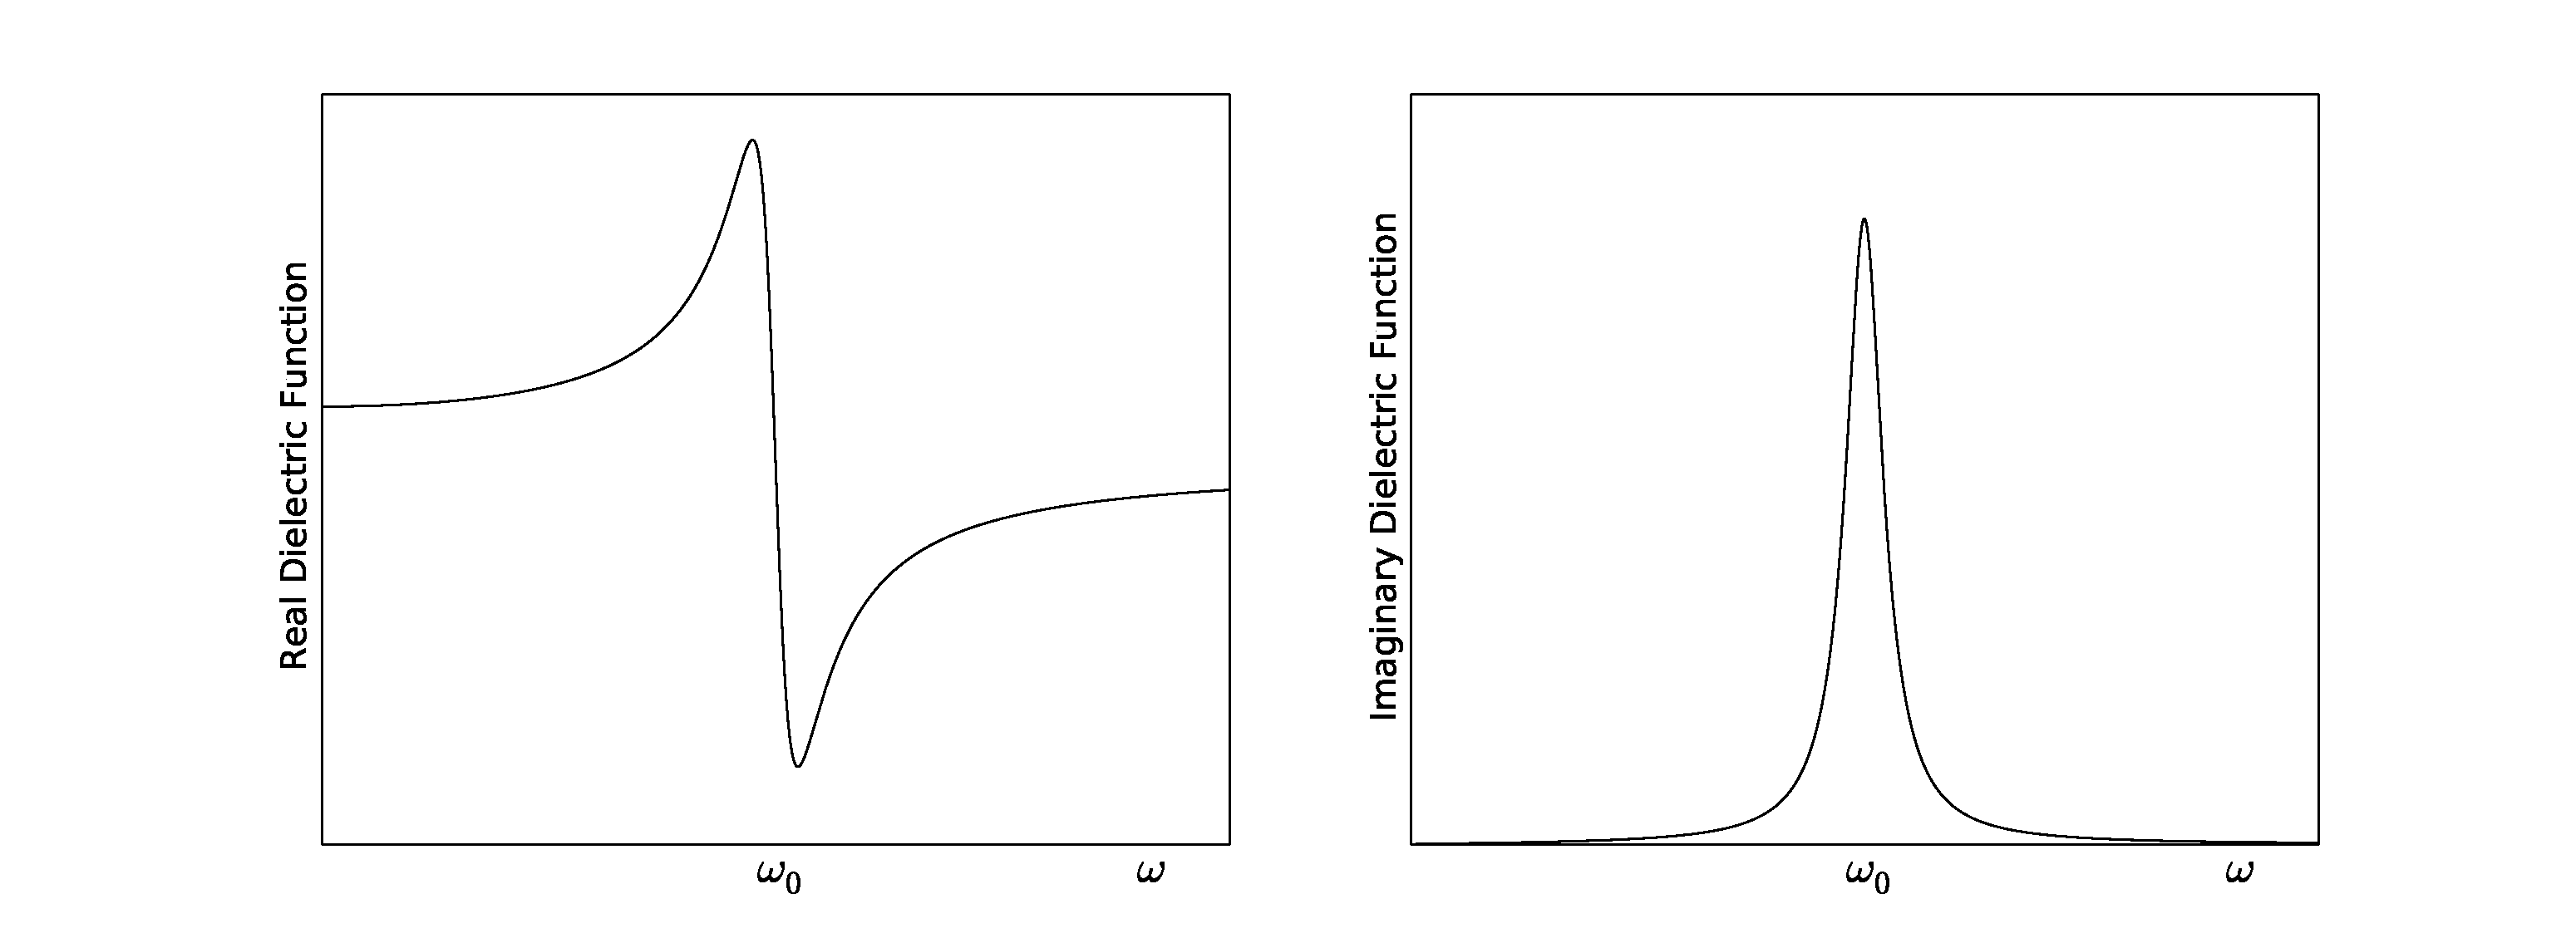
\includegraphics[width=1.0\textwidth]{../Figures/dielectricResonance.pdf}
   \caption{
      The dielectric function of a ionic crystal approximated by
      a driven harmonic oscillator with damping. The left and right figures show the behavior
      of the real and imaginary dielectric function close to
      the resonance frequency $\omega_0$.
   }
   \label{fig:dielectricResonance}
\end{figure}
%
The real part $\varepsilon\!_{_{\Re\! e}} \!\! (\omega)$ is almost constant away from the resonance
frequency, but its value is higher at lower frequencies due to the loss of the contribution from the
ionic polarization. The imaginary part $\varepsilon\!_{_{\Im\! m}} \!\! (\omega)$ is however zero 
everywhere except at the vicinity of the resonant frequency, where it shows a peak with a width
given by the damping coefficient $\eta$. 
\\
\\
To understand the meaning of $\varepsilon\!_{_{\Im\! m}} \!\! (\omega)$ and that the width
if its resonance peak is connected to the damping coefficient $\eta$, one can consider the
energy dissipation in the system. The instantaneous electrical power dissipated per unit 
volume is given by
\begin{align}
   P(t) = j(t)E(t) = j(t)Ee^{- i \omega t}
\end{align}
where j(t) is the curent density. In an insulator, there are no free currents, only polarization currents
\begin{align}
   j(t) = - \frac{\partial D}{\partial t} 
   = - \frac{\partial}{\partial t} \varepsilon \varepsilon_0 Ee^{- i \omega t}
   = i \omega \varepsilon \varepsilon_0 Ee^{- i \omega t}
\end{align}
The average dissipated power is found by averaging over one cycle $T = 2 \pi/\omega$
\begin{align}
   P = \frac{1}{T} \int_0^T E(t)j(t).
\end{align}
If $\varepsilon$ is purely imaginary, $j(t)$ is out of phase with $E(t)$ and their product will always
give a nonzero negative value,$-\varepsilon_0 \varepsilon\!_{_{\Im\! m}} \!\! (\omega) E^2$. On the other
hand, if $\varepsilon$ is purely real, the phase shift will be $\pi/2$ and the integral will give $P = 0$.
$\varepsilon\!_{_{\Im\! m}} \!\! (\omega)$ is therefore a measure of the energy dissipation of the
electric field due to the solid, and is obviously highest at the resonance.
\\
\\
The discussion explains some of the optical behaviour of the material. This is however not the
entire picture. E.g. the frequency dependence in the visible and UV region is not explained here.
These effects are due to the valence electrons, which would need a quantum mechanical description
of the electronic structure of the solid. From the band structure of solids, a qualitative
undestanding is obtainable. Figure \ref{fig:transitionResonance} shows regions of high photon absorbtion
due to the excitation of electrons, and how it is given by the imaginary dielectric function 
$\varepsilon\!_{_{\Im\! m}} \!\! (\omega) ? \varepsilon_i(\omega)$. Note that the photons do not have
enough energy to change the electrons wave vector
%
\begin{figure}[h!]
  \centering
   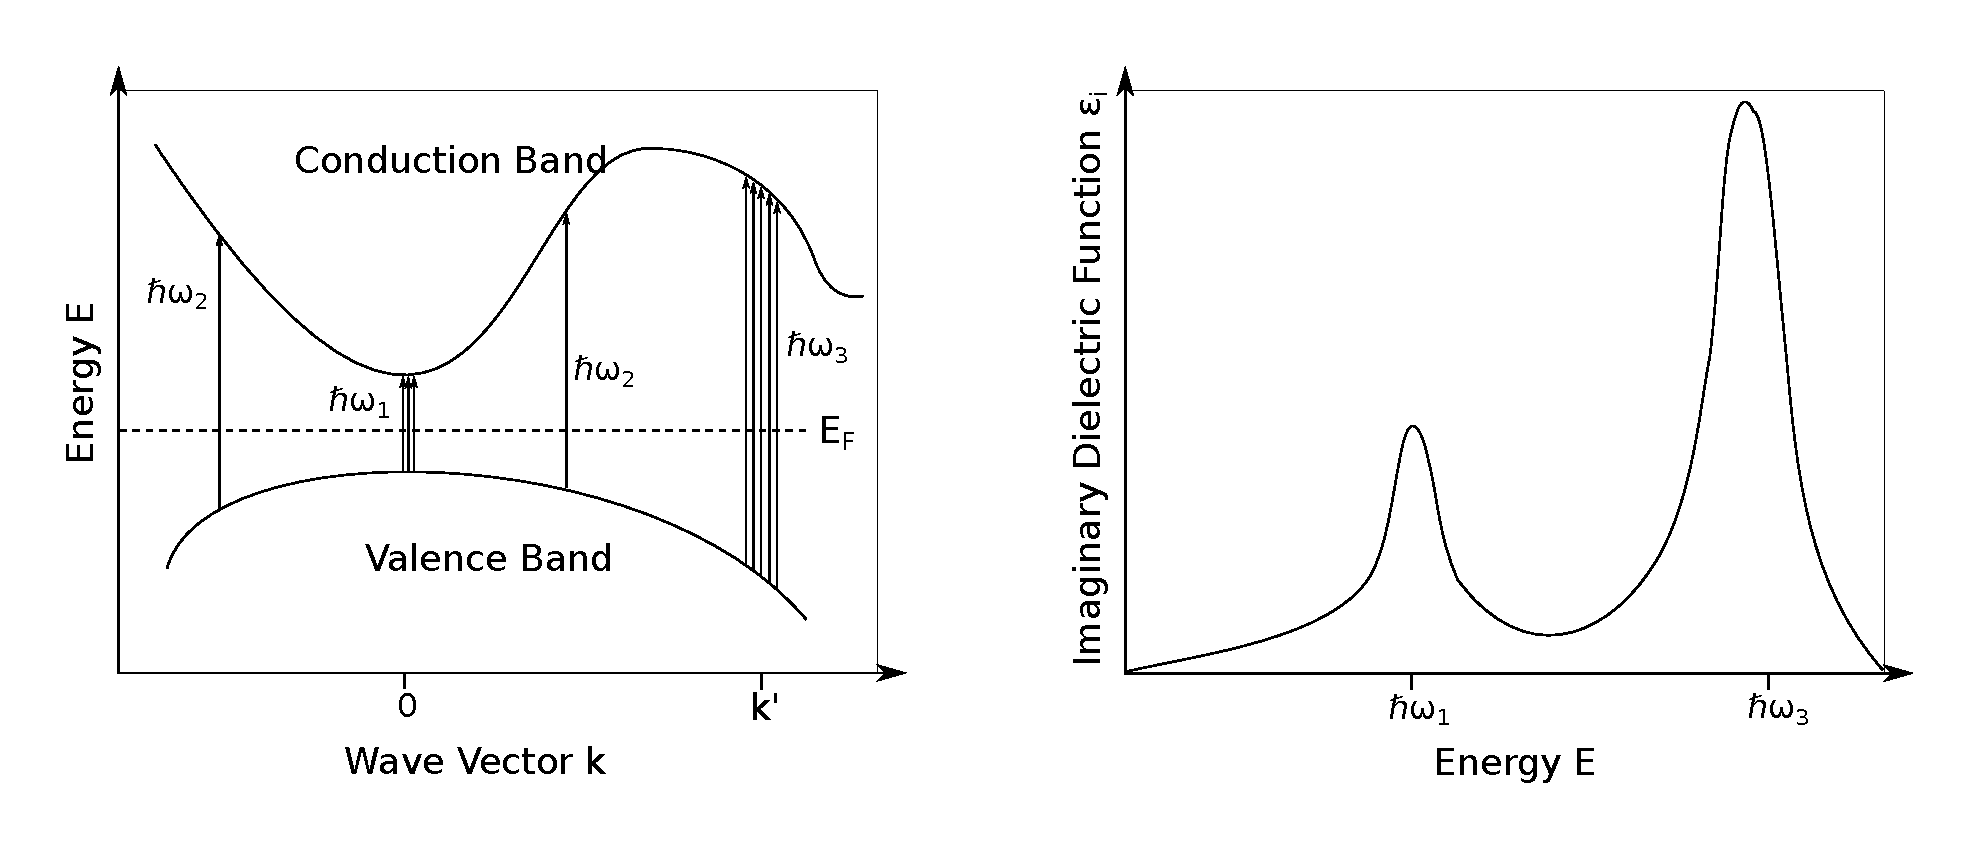
\includegraphics[width=1.0\textwidth]{../Figures/bandstructureVSdielectric.pdf}
   \caption{
      The left figure shows the photon-induced transitions between occupied and unoccupied states in the band 
      structure of a solid. $E_F$ is the fermi energy. 
      In the regions where the valence band and conduction bads are parallel,
      a certain photon energy can excite several states. Here, the parallel regions are located at
      $\boldsymbol k = 0$ and $\boldsymbol k = \boldsymbol k'$ and result in higher transitions density.
      These transitions correspond to absorbtion of the electromagnetic wave given by the imaginary part of
      the dielectric function $\varepsilon_i$. The resulting resonances in $\varepsilon_i$ due to 
      the absorbtion of the $\hbar \omega_1$ and $\hbar \omega_2$ transitions are depicted in the right
      figure.
   }
   \label{fig:transitionResonance}
\end{figure}
%






\begin{thebibliography}{9}

      \bibitem{Hofmann}
         Hofmann P.
         Solid State Physics, An Introduction.
         Wiley-VCH 2008; p.71-74,76-81

\end{thebibliography}




\subsection{Complex permittivity and index of refraction \cite[p.~169-170]{Jensen1985}}
%Jensen B: The Quantum Extension of the Drude-Zener Theory in Polar Semiconductors; p.169-188
The complex dielectric constant or relative permittivity 
$\widehat\varepsilon_r = \varepsilon_r + i \tilde\varepsilon_r$ of a material, is a measure of 
the material's response subject to an electromagnetic field. Here $\varepsilon_r$ and $\tilde\varepsilon_r$ 
denotes the real and imaginary components, respectively.
The relative permittivity is related to
the square of the refractive index, 
\begin{align}
   N^2 = \widehat\varepsilon_r
   \label{compEps}
\end{align}
which determines the optical properties of a given material.
It is like the dielectric constant complex
\begin{align}
   N = n + i k.
\end{align}
The real and imaginary refractive indicies are denotes by $n$ and $k$, respectively
The choice of sign convention, i.e. using $n+ik$ rather than $n-ik$, is determiend by 
the choice of the sign in the in the plane wave solution,
$\exp i(\boldsymbol q \cdot \boldsymbol r - \omega t )$, of
Maxwell's equations.
%The refractive index is also related to the conductivity $\sigma$
%\begin{align}
   %2nk = \frac{4\pi \sigma}{\omega}.
%\end{align}
%
From Eq.\eqref{compEps}
\begin{align}
   \widehat{\varepsilon}_r &= N^2 \\
   \varepsilon_r + i\tilde{\varepsilon}_r &= (n + ik)^2 \\
   \varepsilon_r + i\tilde{\varepsilon}_r &= n^2 - k^2 + i2nk,
\end{align}
and with some simple comparison, the components of the permittivity can be expressed as
\begin{align}
   \varepsilon_r &= n^2 - k^2     &\tilde{\varepsilon}_r  &= 2nk.
\end{align}
Taking the absolute value or modulus,
\begin{align}
   &\big|\widehat\varepsilon_r\big|   = \sqrt{ \varepsilon_r^2 + \tilde{\varepsilon}_r^2} \\
   &\big|\widehat\varepsilon_r\big|   = \sqrt{ (n^2 - k^2)^2 + (2nk)^2} \\
   &\big|\widehat\varepsilon_r\big|^2 = n^4 + 2n^2k^2 + k^4 \\
   &\big|\widehat\varepsilon_r\big|^2 = (n^2 + k^2)^2 \\
   &\big|\widehat\varepsilon_r\big|   = n^2 + k^2,
\end{align}
and putting it all together, gives the real and imaginary parts of $N$ expressed through the 
relative permettivity
\begin{align}
   n      &= \Bigg( \frac{\big|\widehat\varepsilon_r\big| + \varepsilon_r}{2}           \Bigg)^{\frac{1}{2}} 
           %= \Bigg( \frac{\big|\widehat\varepsilon  \big| + \varepsilon}{2\varepsilon_0}\Bigg)^{\frac{1}{2}}
  &k &=      \Bigg( \frac{\big|\widehat\varepsilon_r\big| - \varepsilon_r}{2}           \Bigg)^{\frac{1}{2}} 
           %= \Bigg( \frac{\big|\widehat\varepsilon  \big| - \varepsilon}{2\varepsilon_0}\Bigg)^{\frac{1}{2}}
\end{align}

Considering a plane wave with a complex wave vector $\widehat q = q + i \tilde q$ moving in the material
\cite[p.~402]{Griffiths}
\begin{align}
  e^{i(\widehat q z - \omega t )} 
  = e^{-\tilde q z} e^{i q z - \omega t )} ,
\end{align}
one sees that the wave is attenuated. 
The quantity $\alpha \equiv 2 \tilde q$ is called the absorption coeffiecient
and is proportional to the optical conductivity $\sigma$, to $\tilde\varepsilon$, and to $k$:
\begin{align}
   n\alpha = &\frac{4 \pi \sigma}{c} = \frac{\omega}{c} \tilde\varepsilon\\
                     &\Downarrow \\
   \frac{\alpha}{2} = &\frac{\omega}{c}k = \frac{1}{\delta}
\end{align}
$k$ is usually called the extinction coefficient and is essentially the ratio of the
free-space wave frequency $\omega$ to the skin depth $\delta$.\\


%Experimentally, $n$ and $k$ are found from measurements of the reflectivity R of a bulk, opaque sample
%and the transmittance T of a slab, which are given in terms of $n$ and $k$ as
$n$ and $k$ can be found experimentally by measuring the reflectivity R of a bulk, opaque sample,
in addition to the transmittance T of a slab, which are given in terms of $n$ and $k$ as
\begin{align}
   R &= \frac{(n-1)^2 + k^2}{(n+1)^2 + k^2} \\
   T &= \frac{ (1-R)^2 e^{-2\omega k d / c} }{ 1-R^2 e^{-4\omega k d / c} },
\end{align}
where $d$ is the sample thickness. The slab multiple-reflection effects are averaged,
so that interface fringes are not resolved.
%
\begin{thebibliography}{9}

      %Main article for dielectric function vs refractive index:
      \bibitem{Jensen1985}
       Jensen B.
       The quantum extension of the Drude-Zener theory in polar Semiconductors.
       Handbook of optical constants of Solids, Five-Volume 1997 (1985??)(9)<-it's chapter 9;169-170

      \bibitem{cambdridgePermittivityPage}.
         Dissemination of IT for the promotion of Materials Science (2000)
         Variation of the dielectric constant in alternating fields.
         University of Cambridge 2004:
         http://www.doitpoms.ac.uk/tlplib/dielectrics/variation.php
         (24. August 2015).
         %My interp. of webpage source: 
         %Authors, title, stuff behind(like university?) year ,link (date of site access)
\end{thebibliography}
